\chapter{Idler-frame case study}\label{chap:chapter3}

In this chapter, I apply the methods and learnings from Chap.~\ref{chap:chapter2} to an industry dataset of the failure times of idler-frames on an overland iron ore conveyor. The idler-frames were described briefly in Sec.~\ref{sec:industry-data}. For a reliability engineer tasked with maintaining the conveyor, it can be useful to quantify the expected failure times of the idler-frames currently in operation and the expected number of failures in the next short time interval, such as \citet{hong2009} do for power transformers. I show how these quantities are already naturally contained in the full posterior of the Bayesian model when the censored lifetimes are imputed as in Sec.~\ref{subsec:censoring-treatments}. It is also useful to propagate uncertainty in the posterior estimates of the parameters through any decision criteria to understand risk in long-term maintenance plans, such as the design of a fixed-time replacement strategy. I demonstrate how the joint posterior draws of the Weibull parameters can be propagated through a cost function to make an informed decision about a fixed-time replacement strategy for the idlers in the frames.

The chapter is structured as follows. Section~\ref{sec:idler-frame-data-desc} describes the data in detail. In Sec.~\ref{sec:idler-frame-joint-prior}, I construct an informative prior for the idler-frame analysis based on prior knowledge supplied by the idler manufacturer and a conveyor engineer. Section~\ref{sec:idler-frame-posterior} describes the model fitting process and posterior inference on the parameters. Section~\ref{sec:idler-frames-using-posterior} goes on to demonstrate how the draws from the posterior can be used. Specifically, Sec.~\ref{subsec:idler-FTs} and~\ref{subsec:idler-cumulative-failrues} show how to obtain the estimated remaining useful life of the currently installed idler-frames and the expected number of failures in a time interval following the end of observation, respectively. Sec~\ref{subsec:idler-cost-function} then shows how to propagate the posterior uncertainty about the lifetime distribution through utility functions---specifically a cost function---to inform the choice of a preventative replacement interval for the idler-frames. Finally, Sec.~\ref{sec:idler-frame-conclusions} summarises and concludes the chapter.

\section{Idler-frame lifetime data} \label{sec:idler-frame-data-desc}

The data is a synthesis of preventative and reactive replacement records of idlers on a single overland iron ore conveyor. It is one of many such datasets for similar conveyors on the mine. This specific conveyor has one hundred and forty-three frames of idlers, each with a three-idler configuration. When an idler in the frame fails, all three of the idlers are typically replaced, so each idler frame can be viewed as one unit. The replacements of the idlers in a frame are typically captured in the CMMS, and if an idler in the frame has been observed as failed and scheduled to be replaced, then this information is included in the replacement record. However, if an idler in the frame has failed in a way that threatens to damage the belt immediately, then this is raised in a different system, the belt is shut down, and the idlers in that frame are replaced. During an industry placement, I cleaned and collated these different sources of replacement records into a single dataset. The dataset spans just over six years, but the conveyor has been in operation for twenty.

From the replacement records, the lifetimes of the idler-frames can be calculated as the time between the replacements. However, since the records do not go back to the commissioning of the conveyor, the first observed lifetime for each frame is left truncated and has unknown installation time. Because the sets of idlers in some frames are preventatively replaced or because some were still in operation when I constructed the dataset, there are many right censored lifetimes. Table~\ref{tab:idler-frame-summary} gives an overview of the dataset of idler frame lifetimes, and Fig.~\ref{fig:idler-frames-data} shows the lifetimes of each frame along the conveyor. In Fig.~\ref{fig:idler-frames-data}, the fully observed lifetimes---i.e. we observed the failure of an idler in the frame as well as the previous failure for that frame---are shown as orange points, while the partially observed lifetimes are shown in blue. The partially observed lifetimes that are left-truncated by the beginning of the observation period are shown as triangular points, while the remainder of the blue points are right-censored observations.

\begin{table}
\centering
\caption{\label{tab:idler-frame-summary}Summary of the idler frame data set.}
\centering
\begin{tabular}[t]{ll}
\toprule
\cellcolor{gray!10}{Maximum lifetime} & \cellcolor{gray!10}{2167 days}\\
Minimum lifetime & 1 days\\
\cellcolor{gray!10}{Maximum fully observed lifetime} & \cellcolor{gray!10}{1461 days}\\
Beginning of observation & 2014-12-10\\
\cellcolor{gray!10}{End of observation} & \cellcolor{gray!10}{2020-11-15}\\
\addlinespace
Number of observations & 402\\
\cellcolor{gray!10}{Number of unique frames} & \cellcolor{gray!10}{143}\\
Number of left truncated observations & 143\\
\cellcolor{gray!10}{Number of right censored observations} & \cellcolor{gray!10}{144}\\
Number of left truncated and right censored observations & 1\\
\bottomrule
\end{tabular}
\end{table}


Table~\ref{tab:idler-frame-summary} shows that roughly thirty-six per cent of the lifetimes in the dataset are left-truncated with unknown installation times. Therefore, if we were to discard these observations, we would throw away a third of the data. It is better to retain the information in these left-truncated lifetimes.

Based on our understanding of how the idler-frames fail and from the characteristics of the dataset described in Tab.~\ref{tab:idler-frame-summary}, it is appropriate to use the methods that I developed in Chap.~\ref{chap:chapter2} to analyse the industry dataset and impute the partially observed truncated lifetimes. The Weibull distribution appears appropriate to model the idler-frame lifetimes since the idlers in the frame should fail via a wear-out failure mechanism. Furthermore, the frame's failure time is when the first idler in the frame fails, which aligns with the extreme value distribution characteristic of the Weibull (discussed in Sec.~\ref{subsec:weibull-dist}). The observation period spans just over six years, and it starts roughly 14 years after the conveyor was commissioned. According to domain knowledge, the expected lifetime of an idler is roughly five years, and since the lifetime of a frame is the first of the three idlers to fail, the expected lifetime of a frame should be a little under this value. Hence, the observation window is greater than the expected lifetime, and the time from the commissioning of the conveyor ($t = 0$) to the start of the observation period ($t_{start}$) is roughly three times greater. Furthermore, only one lifetime is left-truncated/interval-censored by the beginning of observation and right-censored by its end. Under these circumstances, it is acceptable to use the methods proposed in Chap.~\ref{chap:chapter2} to account for the lifetimes that are left-truncated with unknown exposure history.

In the industry dataset, there are some very short lifetimes---twenty-five that are less than three weeks---that most likely arise from manufacturing defects or incorrect installation. In this analysis, I aim to model the wear-out failure mechanism of the idler frames, and therefore, I treat any lifetimes shorter than three weeks as right censoring events; this is done by \citet{hong2009} in their analysis of power transformers---i.e. the failure due to wear was right censored by the early failure due to another cause.

\begin{figure}
  \centering
  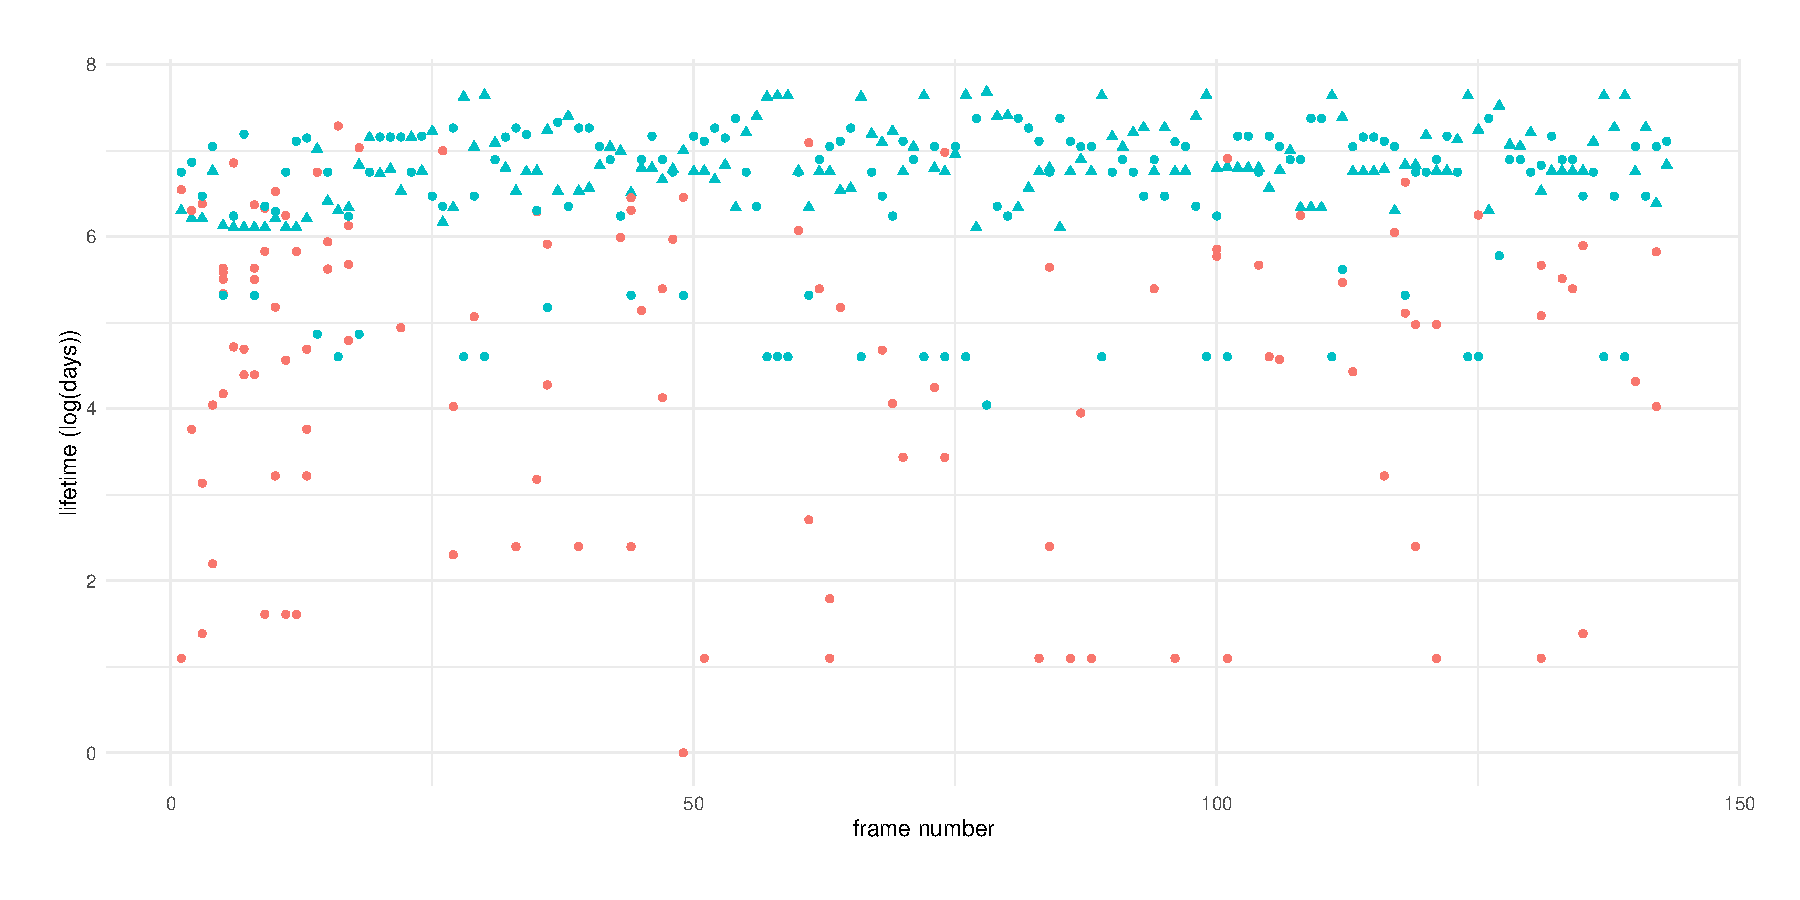
\includegraphics[width=1\textwidth]{./figures/ch-3/idler-frame-data.pdf}
  \caption{The idler-frame lifetimes plotted along the length of the conveyor. On the horizontal axis is the frame number that the lifetimes belong to, and on the vertical is the log value of the lifetime in log-days. The fully observed lifetimes are red points, while the partially observed (censored) lifetimes are blue. The censored lifetimes that are left-truncated by the start of the observation period are shown as triangular points.}
  \label{fig:idler-frames-data}
\end{figure}

\section{An informative prior} \label{sec:idler-frame-joint-prior}

Based on engineering knowledge and information provided by the manufacturer, I construct an informative joint prior for the idler-frames to supplement the analysis. According to the manufacturer, the expected lifetime of an idler is five years, and according to conveyor engineers, it is unlikely that they will last longer than eight. I express this information as the expectation of the CDF at $t_1 = 5 \times 365 = 1825$ and $t_2 = 8 \times 365 = 2920$ encoded as normal distributions, as in Sec.~\ref{sec:weibull-joint-prior}. The expected value of the CDF at $t_1 = 1825$ is $0.50$, and the standard deviation is $0.15$, while the expected value of the CDF at $t_2 = 2920$ is $0.95$ with a standard deviation of $0.05$. I set the standard deviations relatively large since the expected lifetime of a frame of idlers is actually the expected smallest value of the three idlers in the frame. The resulting informative joint prior is shown if Fig.~\ref{fig:idler-frames-prior}, plot~(a) shows three thousand joint draws of the shape $\beta$ and scale $\eta$ from the informative prior, and plot~(b) shows the resulting prior uncertainty in the CDF.

\begin{figure}
  \centering
  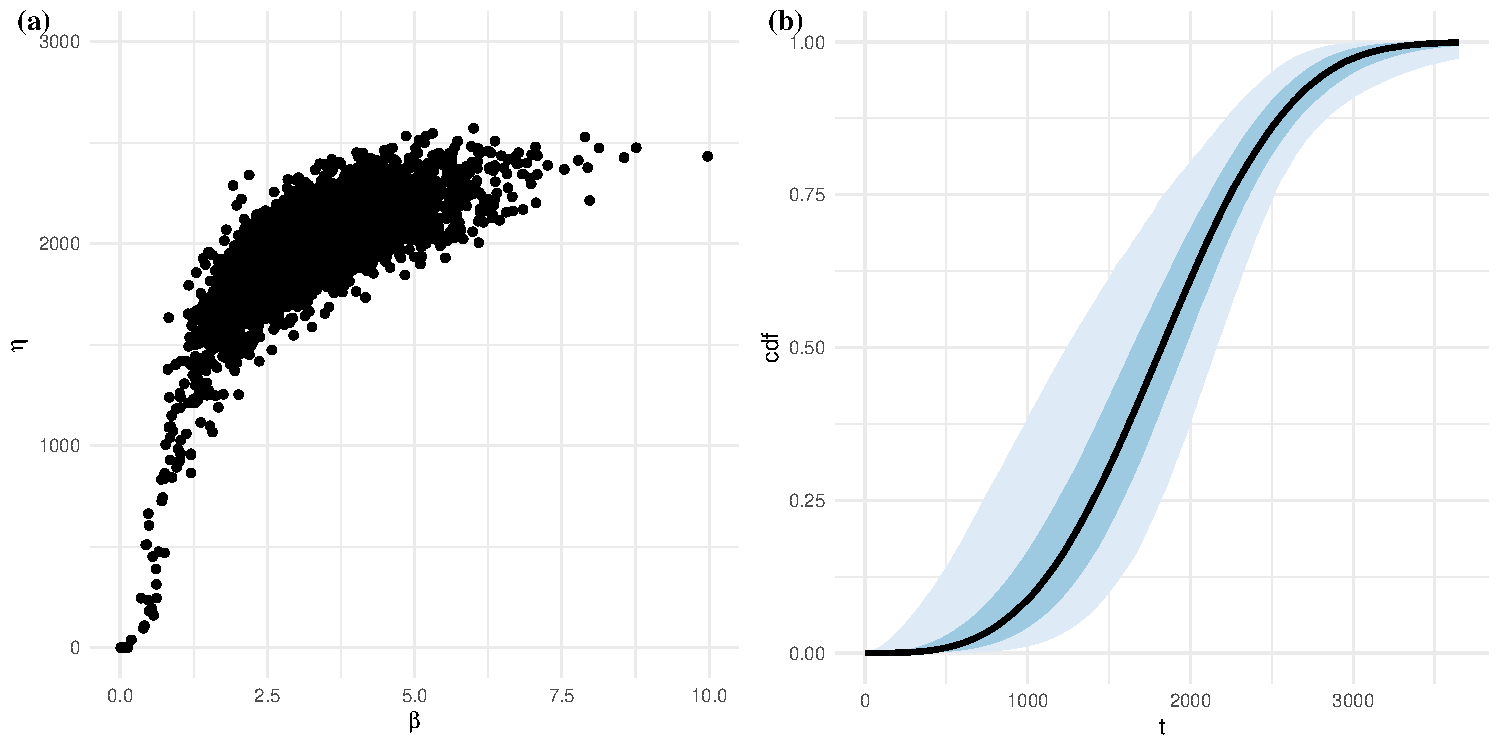
\includegraphics[width=1\textwidth]{./figures/ch-3/idler-frame-prior.pdf}
  \caption{The joint informative prior from eliciting information at $t_1 = 1825$ and $t_2 = 2920$. (a) shows 3000 draws from the informative joint prior, and (b) shows the resulting uncertainty surrounding the CDF.}
  \label{fig:idler-frames-prior}
\end{figure}

\section{Posterior draws} \label{sec:idler-frame-posterior}

To perform inference, I draw $6000$ samples from the posterior using four chains, each $2000$ iterations long and with a burn-in of $500$ iterations and no thinning using Stan \citep{Stan2022}. The Stan output summarising the joint posterior draws of $\beta$ and $\eta$ is shown in Tab.~\ref{tab:idler-frame-posterior-summary} and the joint draws are plotted in Fig.~\ref{fig:idler-frames-post}~(a). Sampling is efficient with no divergences, the chains mix well---indicated by $\hat{R}$ values of $\approx 1$---and both parameters have a large number of effective samples. The posterior mean of the shape is just above one ($1.10$), but there is a small amount of mass just below one, and the posterior mean of the scale is $1363$. These values of the parameters yield an average frame lifetime of $1315$ days or $3.6$ years with $90\%$ lower and upper bounds of $3.2$ years and $3.9$ years, which is significantly smaller than the recommended average lifetime of an idler provided by the manufacturer---which was five years.

\begin{table}
\centering
\caption{\label{tab:idler-frame-posterior-summary}Summary of sampling for $\beta$ and $\eta$.}
\centering
\begin{tabular}[t]{lrrrrrr}
\toprule
Parameter & Mean & 2.5\% & 50\% & 97.5\% & $n_{\small{\mbox{eff}}}$ & $\hat{R}$\\
\midrule
\cellcolor{gray!10}{$\beta$} & \cellcolor{gray!10}{1.10} & \cellcolor{gray!10}{1.01} & \cellcolor{gray!10}{1.10} & \cellcolor{gray!10}{1.20} & \cellcolor{gray!10}{5337} & \cellcolor{gray!10}{1.0001}\\
$\eta$ & 1362.56 & 1200.58 & 1361.17 & 1535.58 & 4386 & 1.0003\\
\bottomrule
\end{tabular}
\end{table}


\begin{figure}
  \centering
  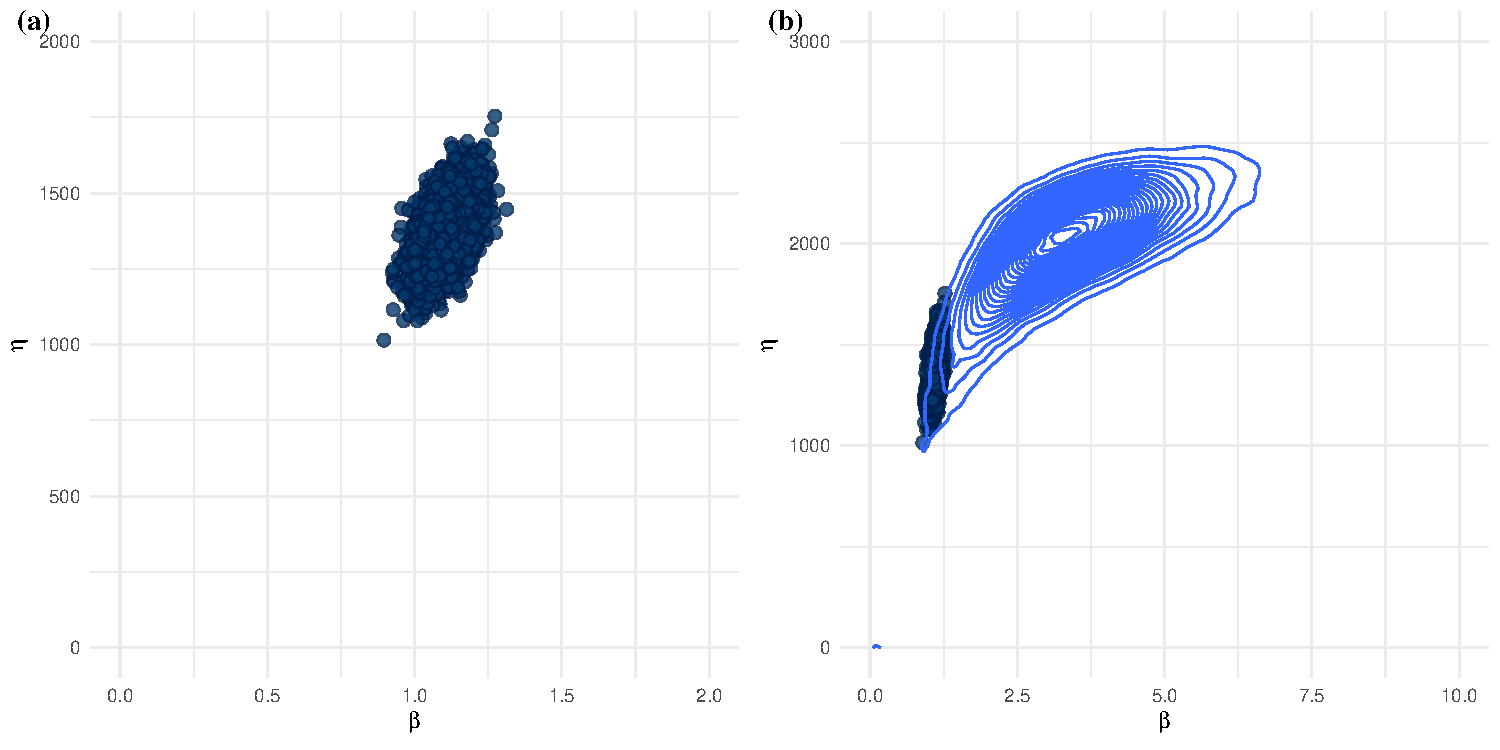
\includegraphics[width=1\textwidth]{./figures/ch-3/idler-frame-post.pdf}
  \caption{The joint draws of the Weibull parameters $\beta$ and $\eta$ from the posterior distribution. (a) shows the plain draws, and (b) compares the draws with the contours of the informative joint prior.}
  \label{fig:idler-frames-post}
\end{figure}

Figure~\ref{fig:idler-frames-post}~(b) compares the draws from the posterior with the informative joint prior. The posterior draws sit far in the tail of the joint prior but are still contained in the prior. The likelihood is strong enough that inference about the shape and scale are fairly invariant to changes in the prior, although I do not show this here. Figure~\ref{fig:idler-frames-post-cdf} shows the refined uncertainty around the CDF that results from the posterior. The uncertainty surrounding the CDF of the lifetime distribution in the figures is much more refined compared with the prior (Fig.~\ref{fig:idler-frames-prior}~(b)). The posterior mean of the CDF at our elicitation times---$t_1 = 1825$ days and $t_2 = 2920$ days---are $0.75$ and $0.90$, respectively. These updated estimates sit in the tails of the distributions I specified to construct the prior. The discrepancy between the prior and the posterior indicates a slight prior-likelihood conflict; however, the likelihood is strong enough, in this case, to not be too influenced by the prior, and the prior does appear to have some mass around the final model.

\begin{figure}
  \centering
  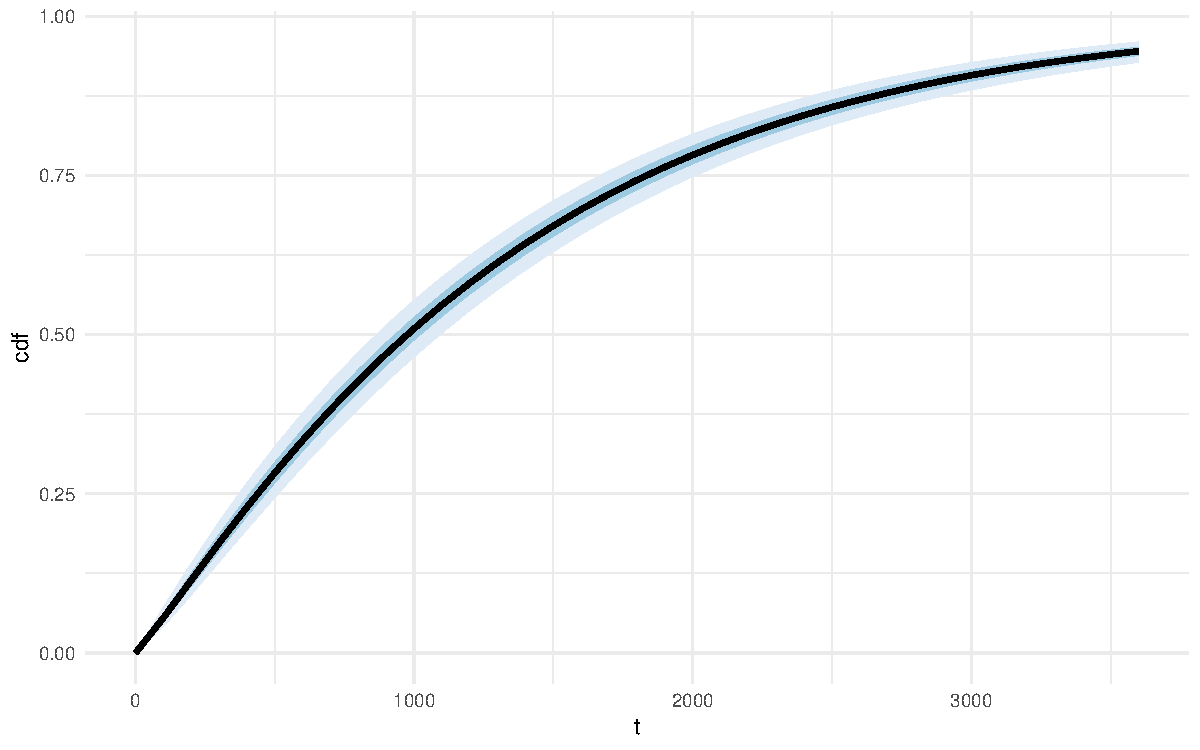
\includegraphics[width=0.7\textwidth]{./figures/ch-3/idler-frame-post-CDF.pdf}
  \caption{The resulting posterior uncertainty surrounding the Weibull CDF.}
  \label{fig:idler-frames-post-cdf}
\end{figure}

\section{Using the posterior} \label{sec:idler-frames-using-posterior}

While the posterior estimates of the parameters are useful in understanding the lifetime distribution, the real value in a Bayesian analysis comes from the uncertainty quantification expressed in the full posterior. Using the draws from the full posterior, which includes the draws of the latent parameters in the model, such as the imputed censored values, we can quantify risk and inform decisions. For example, by imputing the underlying values of the partially observed lifetimes during the MCMC sampling routine, we naturally obtain a distribution for their predicted failure times and consequently can also derive the expected number of failures in the next short time interval. We can also pass the joint draws of the parameters through `utility' functions \citep[Chap.~9]{BDA2020}---for example, a cost function---to incorporate the uncertainty in the analysis into long-term decisions. In this section, Sec.~\ref{subsec:idler-FTs} shows how to obtain predictive distributions of remaining useful life (RUL) for each idler-frame still in operation at the end of the observation period. I then show how these RUL distributions can be used to construct a predictive distribution for the cumulative number of failures going forward from the end of the observation period in Sec.~\ref{subsec:idler-cumulative-failrues}. Finally, Sec.~\ref{subsec:idler-cost-function}, demonstrates how the joint draws of the parameters can be pushed through a cost function to propagate the uncertainty from the analysis and inform the choice of a fixed-time replacement strategy.

\subsection{Failure time of units in operation} \label{subsec:idler-FTs}

In the model for the idler-frame lifetimes, the unobserved values of the censored lifetimes are treated as missing data and their values are imputed, which in a Bayesian framework is to treat them like a parameter in the model. Since I impute the values during the HMC routine, I consequently obtain draws of the imputed values of the censored lifetimes. The distributions of these draws form a predictive distribution missing lifetimes of the right censored units conditioned on their age. This can also be calculated if we were to integrate out the censored lifetimes as discussed in Sec.~\ref{subsec:censoring-treatments} and also if we use maximum likelihood to perform inference, such as \citet{hong2009} do. But in these cases, we would need to calculate the distribution conditional on each censored component's age separately, and if we were to use maximum likelihood, we would need to calculate uncertainty intervals using an appropriate method. It is much more convenient to impute the values in the Bayesian analysis since the estimates and uncertainty for each censored observation are already naturally contained in the posterior.

Using the posterior draws of the imputed lifetimes, I calculate draws of the predicted remaining useful life of each unit still under test by subtracting the censoring time from the imputed value of the lifetime according to
\begin{equation} \label{eq:idler-rul}
  \hbox{RUL}^s_i  = \tilde{y}_{i}^s - c^{\textit{\tiny{Lower}}}_i,
\end{equation}
where $s$ indicates a particular draw from the posterior. The remaining useful life distributions for each of the one-hundred and forty-three frames are shown in Fig.~\ref{fig:idler-FTs}. These distributions can not only be used to obtain point estimates and uncertainty bounds for the RUL, but also order the frames in terms of the highest risk of failure in a particular number of days or, as I show in the next section, determine the expected number of failures within the next short time interval.

\begin{figure}
  \centering
  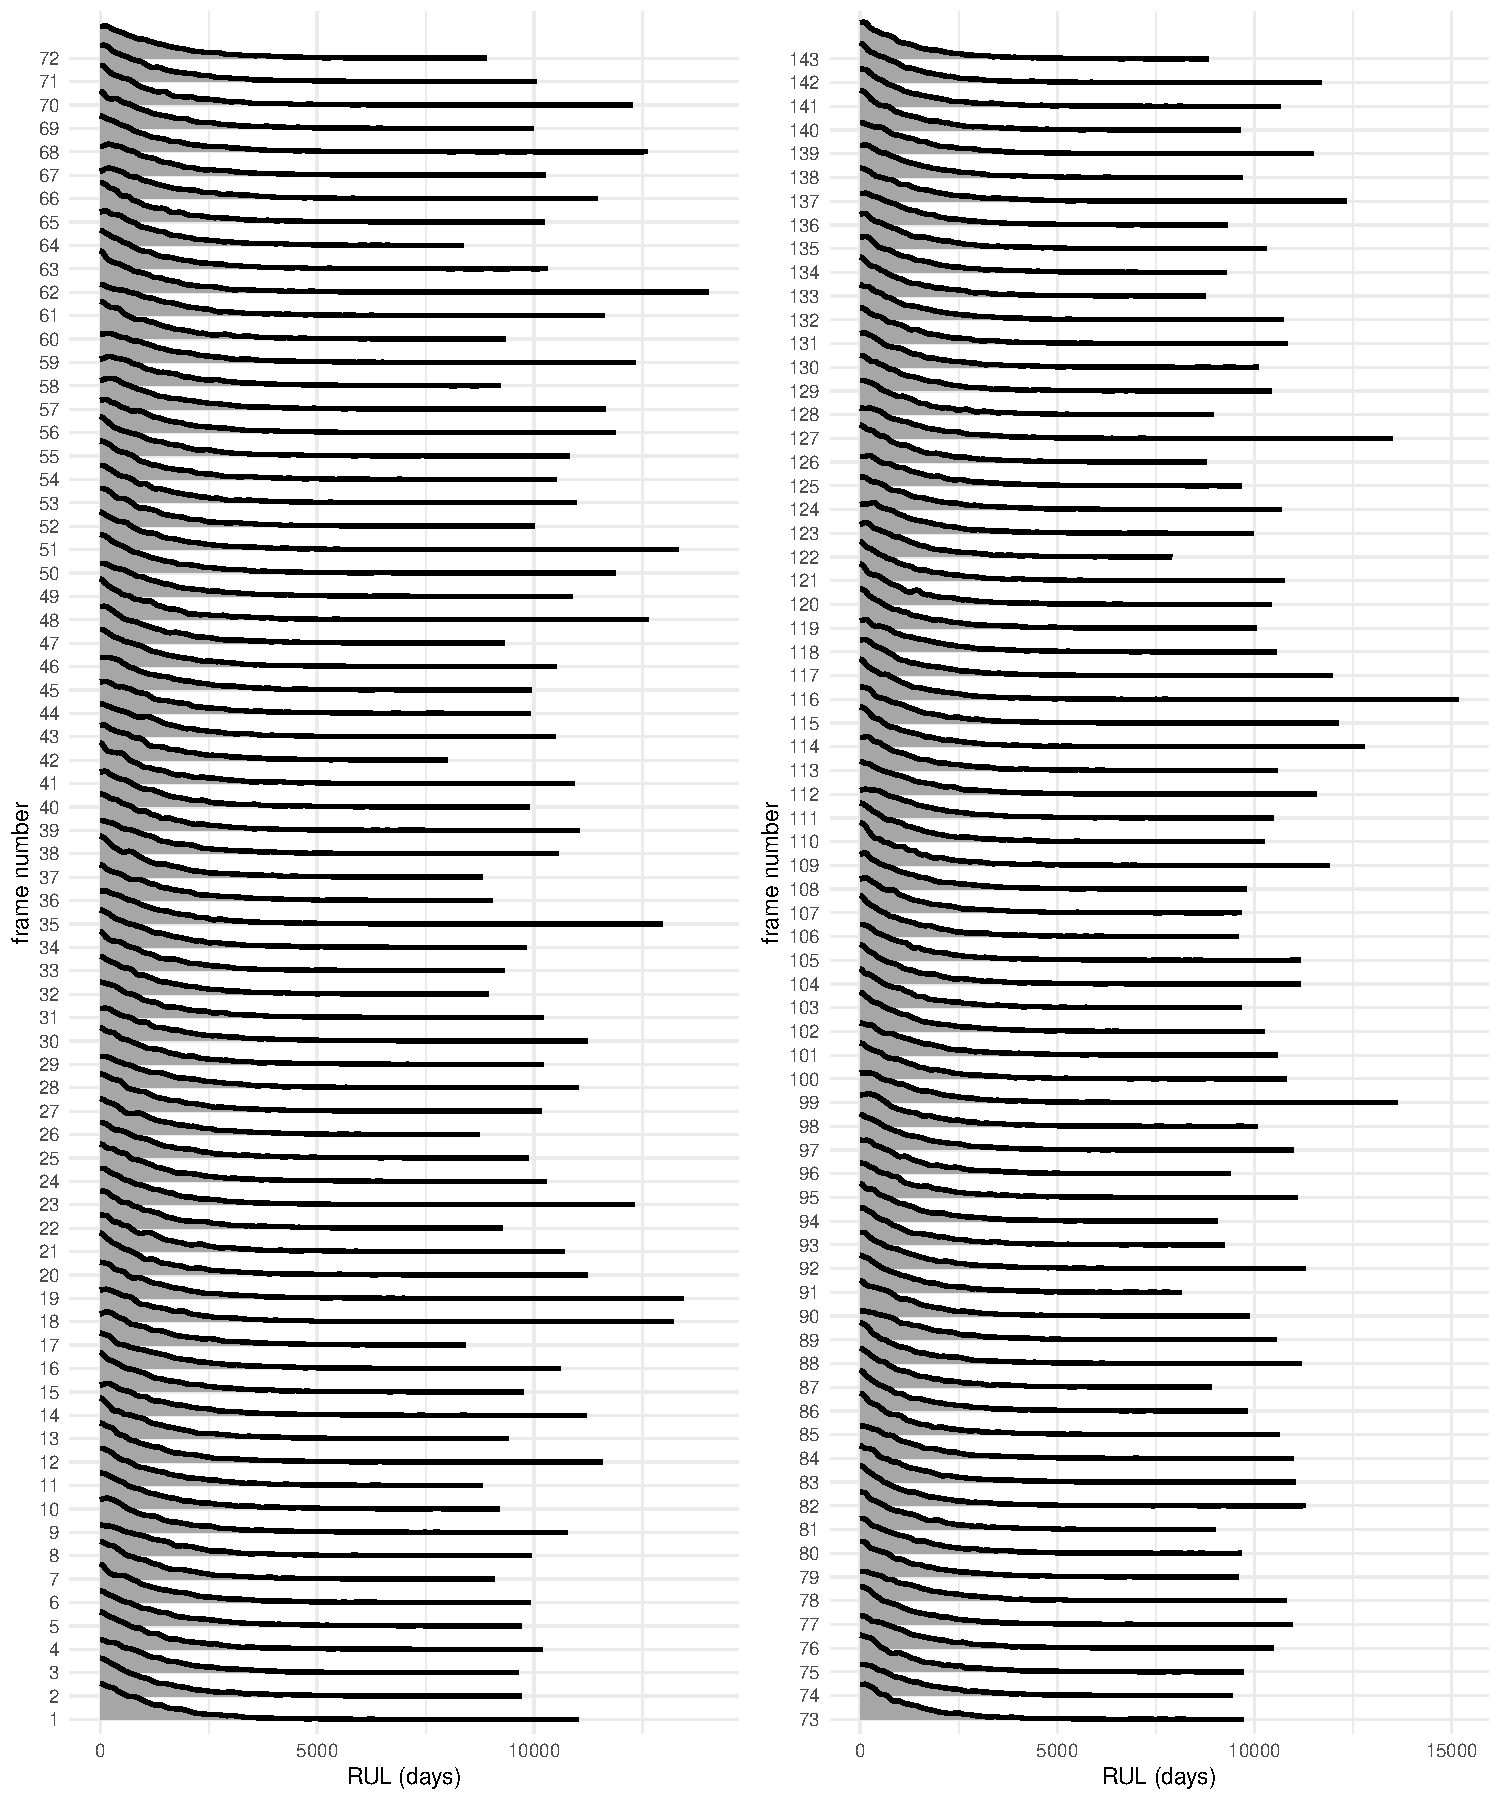
\includegraphics[width=1\textwidth]{./figures/ch-3/posterior-FTs.pdf}
  \caption{The remaining useful life distributions for the current lifetimes (the lifetimes right censored by the end of observation). The left plot shows frames $1$ to $72$, and the right shows frames $73$ through $143$.}
  \label{fig:idler-FTs}
\end{figure}

\subsection{Expected number of failures} \label{subsec:idler-cumulative-failrues}

With each draw from the posterior, I obtain a set of imputed values for the lifetimes of the idler frames still in operation and, with this, a prediction of the remaining useful life. Using the draws of RUL, I can calculate the cumulative failures going forward from the end of the observation period. Using an adaptation of the notation of \citet[sec.~6]{hong2009}, the number of failures at $t$ days from the end of the observation period is $K = \sum^{n}_{i = 1}I_i$, where $I_i = 1$ if $\text{RUL}_i < t$ and $I_i = 0$ if $\text{RUL}_i > t$, and the $\text{RUL}_i$ are calculated as in eq.~\eqref{eq:idler-rul}. I express this step function as $F_K(t|\text{RUL}^s, \theta^s)$ where $\text{RUL} = \{\text{RUL}_1, \dots, \text{RUL}_n\}$. Figure~\ref{fig:E-Nfailrues-draws} shows ten draws of $F_K(t|\hbox{RUL}, \theta)$.

Using the resulting distribution of $F_K(t|\hbox{RUL}, \theta)$, predictive distributions for the number of failures at any time $t$ in the future can be obtained. Figure~\ref{fig:E-Nfailrues-densities} shows the predictive densities for the number of failures within the next one (Fig.~\ref{fig:E-Nfailrues-densities}~(a)), three (Fig.~\ref{fig:E-Nfailrues-densities}~(b)), and six (Fig.~\ref{fig:E-Nfailrues-densities}~(c)) months. From the draws that make up the distributions shown in the figure, it is straightforward to obtain the posterior estimates and uncertainty intervals. Such distributions are useful for managing risk in the short term and planning, for example, managing the inventory of replacement idlers kept on site.

\begin{figure}
  \centering
  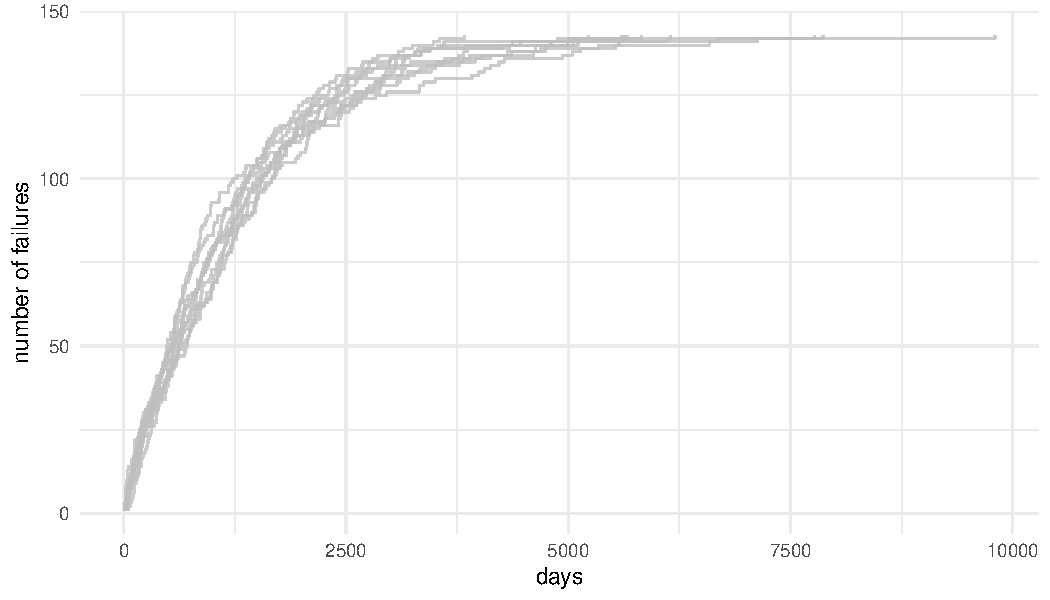
\includegraphics[width=1\textwidth]{./figures/ch-3/E-n-failures-draws.pdf}
  \caption{Ten draws of the cumulative failures proceeding the end of the observation period. The horizontal axis is the days since the end of the observation period, and the vertical axis is the cumulative number of failures.}
  \label{fig:E-Nfailrues-draws}
\end{figure}

\begin{figure}
  \centering
  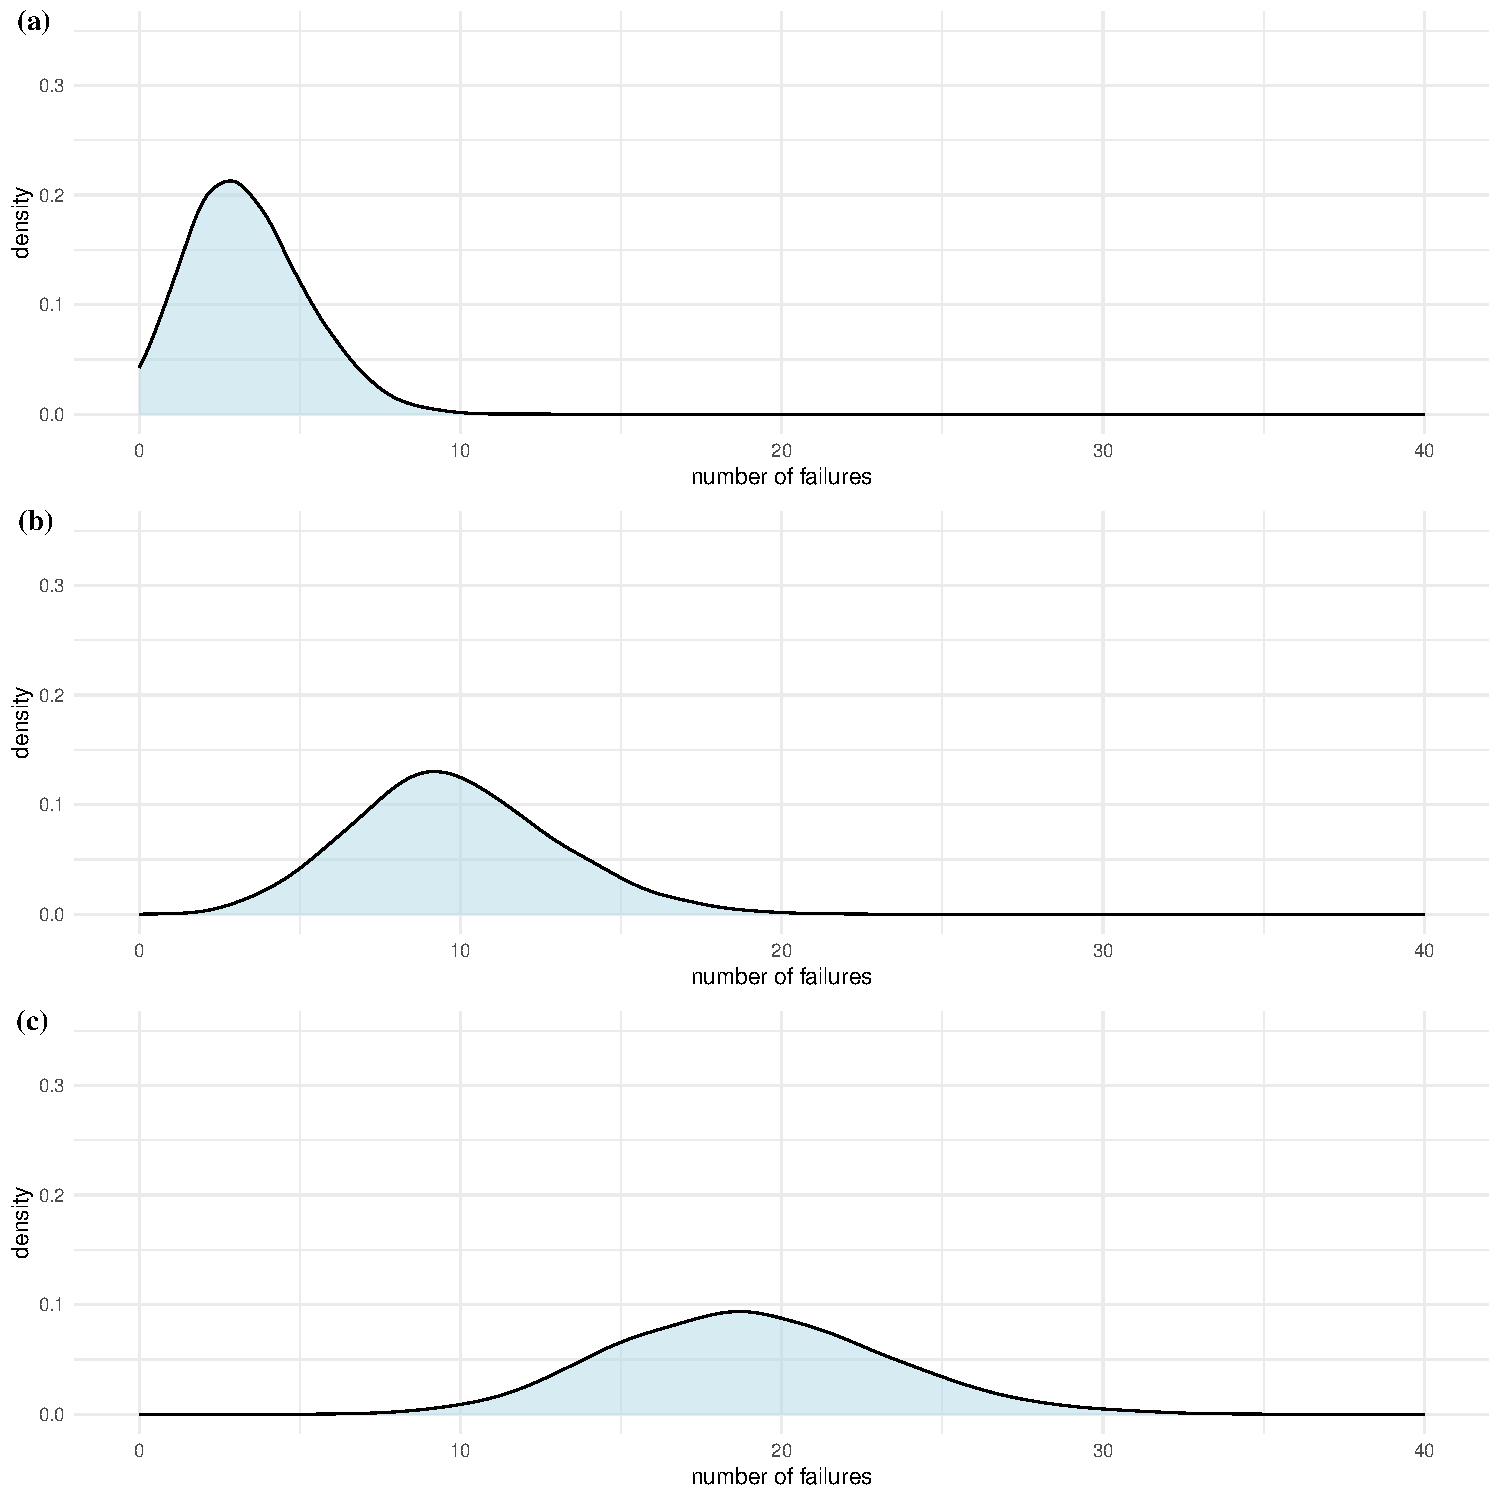
\includegraphics[width=0.7\textwidth]{./figures/ch-3/E-n-failures-densities.pdf}
  \caption{The predictive distributions for the number of failures in the one (a), three (b), and six (c) month period after the end of the observation period.}
  \label{fig:E-Nfailrues-densities}
\end{figure}

\subsection{Cost functions and preventative policy design} \label{subsec:idler-cost-function}

The posterior draws are not only useful for making short-term decisions, functions of the draws of the parameters can inform long-term planning. As an example, in this section, I incorporate the posterior uncertainty in the parameters into the choice of fixed time replacement interval for a preventative maintenance policy.

To implement a preventative replacement strategy, a reliability practitioner must choose a fixed time interval at which components are replaced. This choice aims to minimise the expected cost of maintenance and lost production but must also align with what is practically possible. \citet{jardine2013} propose a rough structure for quantifying the cost of a particular preventative maintenance policy according to
\begin{equation*}
 \textit{Cost per unit time} = \frac{C_p N + C_r E[K|\Delta t_p,\theta]}{\Delta t_p},
\end{equation*}
which balances the cost of planned replacements $C_p$ against the cost of unplanned (reactive) replacements $C_r$ in terms of cost per unit time. $N$ is the number of units covered by the scheme, $\Delta t_p$ is the proposed fixed time interval, and $E[K|\Delta t_p,\theta]$ is the expected number of reactive maintenance events in the interval given the parameters of the lifetime distribution. Since the cost due to reactive maintenance depends on the lifetime distribution, we should incorporate the uncertainty around the parameters of this distribution.

Here, I give a general example of propagating posterior uncertainty through a cost function for the idler-frames bulk replacement. Let $\Delta t_p$ denote the time interval between bulk replacements of the idler-frames analysed in Sec.~\ref{sec:idler-frame-posterior}. The cost to replace an idler in a bulk replacement during a shutdown period is $\approx\$250$ per idler, that is $\approx\$750$ per frame. However, if an idler needs to be replaced during a period of operation, this costs $\approx\$2,000$ in parts and labour and typically takes around two hours. Critical conveyors in the circuit will transport around $15000$ tonnes/hour. At a conservative iron ore price of $\$100$ a tonne, a two-hour stoppage equates to $\$3,000,000$ in lost production. The cost function for the bulk replacements of the idlers is therefore
\begin{equation*}
 \textit{Cost per unit time} = \frac{\$750 \times 143 + (\$3,000,000 + \$2,000) E[K|\Delta t_p,\beta,\eta]}{\Delta t_p}.
\end{equation*}
Here, because the expected number of unplanned replacements in the interval, $E[K|\Delta t_p,\beta,\eta]$, depends on the posterior values of the parameters $\beta$ and $\eta$, $E[K|\Delta t_p,\beta,\eta]$ is a random variable, and as a result, so too is the \textit{cost per unit time}. Samples from the distribution of \textit{cost per unit time} are obtained by calculating $E[K|\Delta t_p,\beta^s,\eta^s]$, conditioning on each draw from the posterior. However, It is slightly more complicated to calculate this value for the idlers than in the examples provided in \citet{jardine2013}.

\paragraph*{Expected number of reactive maintenance events}

The expected number of reactive maintenance in an interval is non-trivial for two reasons. First, the idlers are repeatedly replaced when they fail, and secondly, not all idler-frame failures will need to be replaced immediately, only those that fail in a way that poses an immediate threat to the belt. The expected number of failures, therefore, needs to be approximated numerically. Section~2.4.3 of \citet{jardine2013} discusses some methods to determine the expected number of repeat failures in a time interval for more straightforward cases and here I describe a method for the idler frames when not all unplanned failures result in reactive maintenance and inflated costs.

In the idler-frame problem, planned and non-urgent maintenance is only performed during shutdowns every six weeks. I therefore confine my simulations to discrete values of $\Delta t_p$, which are multiples of six weeks, ranging from one to forty-four shutdowns (five years). For each draw of $\beta$ and $\eta$ from the posterior, I run one thousand simulations, iteratively simulating the failures in the periods between shutdowns, going up to forty-four. This process is described in Alg.~\ref{algo:K_RM}. Each simulation run reflects the typical workflow on the mine; frames fail in the period between shutdowns and, unless they are an immediate threat to the belt, are flagged and maintained in the next shutdown. However, if an idler in the frame fails in a way that immediately threatens to damage the belt, then the conveyor is stopped and the idlers in that frame replaced, which is when the high reactive maintenance cost is incurred. Therefore, in the simulation runs, starting with all frame ages of zero, I simulate the number of failures in the interval between shutdowns by summing $N$ independent Bernoulli trials
\begin{align*}
 I_n|\Delta t_{shuts}, t_n, \beta^s, \eta^s \sim & \mbox{Bernoulli}(P_{n}) \\
 K_{\text{UF}} = & \sum^N_{i = 1} I_i
\end{align*}
where $P_{\text{UF} n}$ is calculated according to the Weibull lifetime distribution
\begin{equation*}
 P_{\text{UF} n}|\Delta t_{shuts}, t_n, \beta^s, \eta^s = \frac{F_{\text{Weibull}}(t_n + \Delta t_{shuts}|\beta^s, \eta^s) - F_{\text{Weibull}}(t_n|\beta^s, \eta^s)}{1 - F_{\text{Weibull}}(t_n|\beta^s, \eta^s)}.
\end{equation*}
$t_n$ is the age of the frame in days at the beginning of the interval, and $\Delta t_{shuts} = 6 * 7$ days is the period between shutdowns. During the operational periods, I assign a probability $P_{\text{RM}} = 0.05$ that an unplanned frame failure must be replaced immediately. The number of reactive maintenance events in a period between two shutdowns is, therefore, a binomial trial with sample size $K_{\text{UF}}$
\begin{equation*}
 K_{\text{RM}}|\Delta t_{shuts}, t_n, \beta^s, \eta^s \sim Binomial(K_{\text{UF}}, P_{\text{RM}}).
\end{equation*}
At the end of each step (the period between shutdowns), I reset the age of any failed frames to zero, progress the surviving frames ages by $t_{shuts}$ and then move to the next step and repeat the same process.

\begin{algorithm}
	\caption{Numerical procedure to calculate the expected cumulative number of reactive maintenance events. For each draw from the posterior, $1000$ simulations are run, each $44$ shutdowns long.}
  \label{algo:K_RM}
	\begin{algorithmic}[1]
    \State Assign simulation parameters
    \State $N_{\text{frames}} \gets 143$         \Comment{\small{Number of frames}}
    \State $N_{\text{shuts}} \gets 100$          \Comment{\small{Number of shutdowns to run each simulation for}}
    \State $N_{\text{runs}} \gets 1000$          \Comment{\small{Number of runs of the simulation}}
    \State $\Delta t_{shuts} \gets (6 \times 7)$ \Comment{\small{Operating days between shutdowns}}
    \State $P_{\text{RM}} \gets 0.05$            \Comment{\small{Operating days between shutdowns}}
    \State
		\For {every fifth posterior draw $s = 1:5:S$}
      \For {$i = 1$ to $N_{\text{runs}}$}
        \State $t_1, \dots, t_N \gets 0$         \Comment{\small{Set age of frames to zero}}
        \For {$j = 1$ to $N_{\text{shuts}}$}
          \State Calculate probability of frame failures in period between shutdowns.
          \State $P_{\text{UF} n} \gets \frac{F_{\text{Weibull}}(t_n + \Delta t_{shuts} | \theta^s) - F_{\text{Weibull}}(t_n | \theta^s)}{1 - F_{\text{Weibull}}(t_n | \theta^s)}$
          \State $I_n \sim \mbox{Bernoulli}(P_{\text{UF} n})$   \Comment{\small{Simulate frame failures}}
          \State $K_{\text{UF}} \gets \sum^N_{n = 1} I_n$       \Comment{\small{Number of frame failures}}
          \State $K_{\text{RM}|\Delta t_{shuts}}[j] \sim \mbox{Binom}(K_{\text{UF}}, P_{\text{RM}})$ \Comment{\small{Number of reactive maintenance events}}
          \For {$n = 1$ to $N$}
            \If {$I_n = 1$}
              \State $t_n \gets 0$   \Comment{\small{Reset age of failed frames to 0}}
            \Else
              \State $t_n \gets t_n + \Delta t_{shuts}$   \Comment{\small{Progress age of unfailed frames}}
            \EndIf
          \EndFor
        \EndFor
        \State Take Cumulative sum of the reactive maintenance events over the $N_{\text{shuts}}$ periods between shutdowns.
        \State $K_{\text{RM}|t} \gets \text{cumulative sum of } K_{\text{RM}|\Delta t_{shuts}}$
      \EndFor
    \State Average across the simulation runs
    \State $E[K_{\text{RM}|t}]$
    \EndFor
	\end{algorithmic} 
\end{algorithm} 

In each run, at the end of the forty-four shutdowns, I calculate the cumulative number of reactive maintenance events, and at the end of the one-thousand repeat simulations for a draw, I calculate the average for each of the forty-four intervals across the simulations. The result is an approximation of the function for the average number of reactive replacements conditioned on the draw from the posterior by times $\Delta t_p = \{6, 12, \dots, 264\}$ weeks.

Algorithm~\ref{algo:K_RM} is computationally intensive, and so I thin the draws from the posterior, using only every fifth draw. The resulting draws of $E[K_{\text{RM}}|\Delta t_p,\theta^s]$ approximate the distribution of the average cost per unit time for the deferent choices of fixed time replacement intervals.

\paragraph*{Choosing a fixed time replacement interval}

Figure~\ref{fig:preventative-repl-decision} shows the predictive distribution of \textit{cost per unit time} for the different choices of fixed time replacement intervals going up to five years along with the median and $50\%$ and $90\%$ intervals of the distributions. Importantly, the distributions provide the range from the `best case scenario' to the `worst case scenario' of the average cost for a chosen fixed time replacement interval based on the posterior uncertainty. In the figure, when the fixed time interval is greater than 150 weeks, bulk replacements stop having much of an impact on the \textit{cost per unit time}, which makes sense considering that the posterior expectation of an idler-frame lifetime is around three and a half years (185 weeks). The biggest potential cost savings are for the fixed time replacement intervals less $\le 60$ weeks.

\begin{figure}
  \centering
  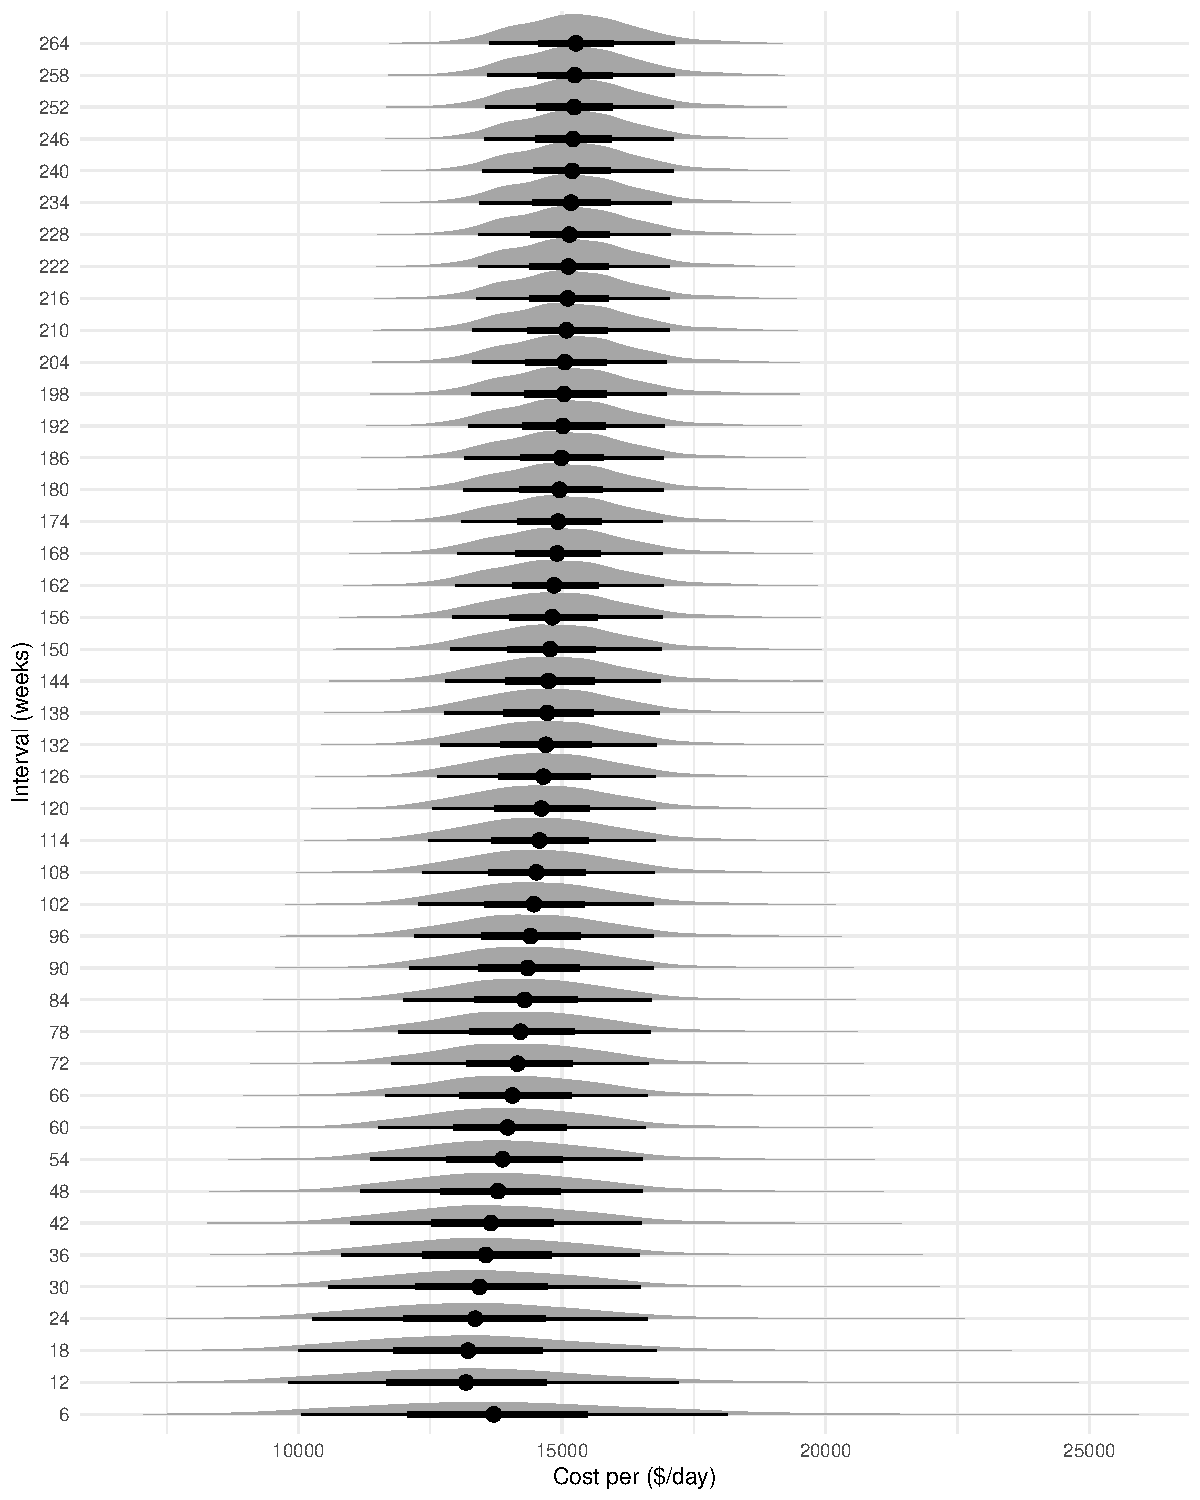
\includegraphics[width=0.8\textwidth]{./figures/ch-3/cost-funciton.pdf}
  \caption{The cost per unit time of preventative maintenance policies for idlers. On the horizontal axis is the cost per unit time, and on the vertical is the fixed time replacement interval. The point and intervals show the median and $0.5$ and $0.9$ intervals. The grey densities show the full distributions.}
  \label{fig:preventative-repl-decision}
\end{figure}

Table~\ref{tab:cost-per-unit-time} summarises the predictive distributions for the ten shortest fixed time intervals. 
The fixed time interval with the smallest potential cost per day is $\Delta t_p = 12$ weeks (every two shutdowns) since the lower $90\%$ uncertainty bound is only $\$9,818$ per day---in other words 
\begin{equation*}
 \text{Pr}\left[\textit{cost per unit time} < \$9,818 | \Delta t_p = 12 \: \text{weeks}, \text{DATA} \right] = 0.05.
\end{equation*}
However, the uncertainty around the lifetime distribution also means that replacing the idlers in the frames every twelve weeks could be over-maintaining the idler-frames since the upper bound of the $90\%$ uncertainty interval at $\Delta t_p = 12$ weeks is the second largest, after $\Delta t_p = 6$ weeks.

\begin{table}
\centering
\caption{\label{tab:cost-per-unit-time}Summary of predictive distributions of cost per unit time (in \$/day).}
\centering
\begin{tabular}[t]{rrrrrrrr}
\toprule
Interval (weeks) & Mean & 5\% & 25\% & 50\% & 75\% & 95\% & $\text{Pr}[< \$15000]$\\
\midrule
\cellcolor{gray!10}{6} & \cellcolor{gray!10}{13857} & \cellcolor{gray!10}{10059} & \cellcolor{gray!10}{12060} & \cellcolor{gray!10}{13704} & \cellcolor{gray!10}{15491} & \cellcolor{gray!10}{18135} & \cellcolor{gray!10}{0.69}\\
12 & 13273 & 9818 & 11677 & 13178 & 14714 & 17216 & 0.79\\
\cellcolor{gray!10}{18} & \cellcolor{gray!10}{13267} & \cellcolor{gray!10}{10000} & \cellcolor{gray!10}{11811} & \cellcolor{gray!10}{13217} & \cellcolor{gray!10}{14622} & \cellcolor{gray!10}{16792} & \cellcolor{gray!10}{0.80}\\
24 & 13369 & 10270 & 11985 & 13352 & 14688 & 16613 & 0.80\\
\cellcolor{gray!10}{30} & \cellcolor{gray!10}{13498} & \cellcolor{gray!10}{10575} & \cellcolor{gray!10}{12219} & \cellcolor{gray!10}{13434} & \cellcolor{gray!10}{14724} & \cellcolor{gray!10}{16480} & \cellcolor{gray!10}{0.79}\\
\addlinespace
36 & 13615 & 10813 & 12362 & 13553 & 14792 & 16461 & 0.78\\
\cellcolor{gray!10}{42} & \cellcolor{gray!10}{13725} & \cellcolor{gray!10}{10984} & \cellcolor{gray!10}{12516} & \cellcolor{gray!10}{13649} & \cellcolor{gray!10}{14844} & \cellcolor{gray!10}{16498} & \cellcolor{gray!10}{0.77}\\
48 & 13833 & 11175 & 12694 & 13784 & 14965 & 16519 & 0.76\\
\cellcolor{gray!10}{54} & \cellcolor{gray!10}{13930} & \cellcolor{gray!10}{11362} & \cellcolor{gray!10}{12806} & \cellcolor{gray!10}{13872} & \cellcolor{gray!10}{15016} & \cellcolor{gray!10}{16525} & \cellcolor{gray!10}{0.75}\\
60 & 14019 & 11526 & 12933 & 13968 & 15088 & 16588 & 0.73\\
\bottomrule
\end{tabular}
\end{table}


The safer choices are the fixed time interval with the lowest risk of over-maintaining the idler-frames. For example the upper bound of the $90\%$ intervals for $\Delta t_p = 30$, $36$, and $42$ weeks are $\$16,480$, $\$16,480$, and $\$16,498$ per day, respectively. These choices offer reduced costs---although possibly not the largest reduction---and the reasonably large replacement intervals are desirable because they provide flexibility when planning the replacement work around the maintenance of other assets---i.e. they would not take up less of the collective labour resources.

Another way that the fixed time interval could be chosen is based on some criteria, e.g. the highest probability that the cost will be less than $\$15,000$ a day, in other words, the minimum $\text{Pr}\left[\textit{cost per unit time} < \$15,000 | \Delta t_p, \text{DATA} \right]$. The rightmost column in Tab.~\ref{tab:cost-per-unit-time} shows this probability for each fixed time interval. Based on this criterion and the posterior uncertainty around the lifetime distribution, the most suitable fixed time interval is either 18 or 24 weeks. However, 12-48 weeks all have very similar probabilites and so are all reasonable choices, and the final decision depends on the wider context of maintenance planning at the mine. Note that these conclusions would differ for different conveyors since their reliability, the cost of maintaining them, and their impact on production may differ. 

Lastly, in the cost function I have used, I have looked only at the expectation of the number of reactive maintenance events; I do not include the variability. It may also be important to investigate the variability in the cost over a short period. For example, the cost of preventative maintenance over a short period should always be roughly the same, whereas the cost due to reactive maintenance may vary a lot. Therefore, it may be preferable to favour shorter fixed-time replacement intervals if it reduces the risk of large financial costs incurred over a short period of time.

\section{Discussion and conclusions} \label{sec:idler-frame-conclusions}

In this chapter, I have demonstrated my proposed method for modelling lifetime data that are right censored and left truncated with unknown exposure time from Chap.~\ref{chap:chapter2} on an industry dataset of idler-frame failure times. From the output of the Bayesian model that imputes the partially observed lifetimes, I showed how it is easy to obtain predictive distributions (and therefore point estimates and uncertainty intervals) for the remaining useful life of the units still in operation at the end of the observation period as well as the cumulative number of failures going forward from the end of the observation period. I also showed how to pass the posterior draws of the Weibull parameters through a cost function to choose a fixed time replacement interval for a preventative maintenance policy in a way that accounts for the posterior uncertainty in the analysis. In this last section, I discuss the main conclusions and outcomes from the chapter and the potential for future work. 

According to the analysis in Sec.~\ref{sec:idler-frame-posterior}, the an idler-frame is $3.6$ years (with 90\% lower and upper bounds of 3.2 and 3.9 years). This estimate is shorter than the prior belief about the expected lifetime of an idler provided by the manufacturer, which is a sign of conflict between the prior and the data. Possible reasons for this conflict are 1) because the analysis I perform is at the frame level since failures are not reliably reported at the idler-level, and 2) the analysis is performed with respect to calendar date. A better exposure would be throughput or travel of the belt since these more strongly indicate usage; however, only calendar time was available.

I demonstrated, using the posterior draws, that imputing the partially observed lifetimes---in particular the right-censored lifetimes---in a Bayesian approach provides a very natural and straightforward way of obtaining estimates and uncertainty intervals for the RUL of the frames still in operation and the predicted cumulative number of failures. The Bayesian approach, therefore, alleviates the analyst from choosing a suitable method for generating uncertainty intervals. The predictive distributions of the RUL of the idlers can be used to prioritise replacements, and the predictive distribution of the cumulative number of failures---derived from the distributions of RUL---can help with logistics; for example, many mines are remote, so they can only hold a particular amount of stock on site, knowing a range for the possible number of failures in the next month would help decide how many replacement idlers should be kept on site.

I have shown that analysis of the partially observed idler-frame lifetimes is useful for short and long-term decisions. However, this could be improved further by including extra information. For example, there is extra information for the idlers, such as manufacturer type---which is available for the recent idler failures---or the location on the belt---idlers in the impact zone where ore is loaded onto the belt or idlers near the head or tail of the belt where were it transitions onto the pulleys. This information could be included through covariates or used to divide the population into groups of similar but different idler-frames, and these groups modelled hierarchically in the Bayesian model. Furthermore, in my analysis, I treated short lifetimes where $t < 21$ days as right censoring events. These early failures can still result in downtime of the belt. Methods could be explored to include these `infant mortalities' in the model, e.g. using a mixture distribution such as in \citep{mittman2013}. However, such an extension would need to investigate the impacts on the imputation of the partially observed lifetimes and missing truncation times.

In this case study analysis of the idler-frame failures, I have emphasised how the posterior can inform decisions. This extension of the discussion of Bayesian analysis of lifetime data is useful for people applying these methods in practice. Rather than taking the point estimates of the quantities of interest and `plugging' them into some utility function, one of the biggest benefits of the Bayesian framework is how easy it is to propagate uncertainty through these types of functions. It is important to emphasise this in work that targets reliability practitioners.